\documentclass[10pt]{beamer}

\newcommand{\lectnum}{L07}
\newcommand{\lecttitle}{Regresssion and Classification Trees}

\usepackage{amsmath, amssymb, graphicx}
\usepackage[]{algorithm2e}
\usepackage{pdfpages}
\usepackage[british]{babel}

\hypersetup{colorlinks,linkcolor=,urlcolor=blue}
\newenvironment{titledslide}[1]{\begin{frame}\frametitle{#1}}{\end{frame}}

\mode<presentation>{\setbeamercovered{transparent}}

\setbeamertemplate{sidebar right}{}
\setbeamertemplate{footline}{%
\hfill\usebeamertemplate***{navigation symbols}
\hspace{0.4cm}\lectnum: \insertframenumber{}/\inserttotalframenumber \hspace*{0.4cm}}

\author{James Cussens}

\title{COMS30035, Machine learning:\\ \vspace{5pt} \lecttitle}

\institute{School of Computer Science\\University of Bristol}

\begin{document}
%%%%%%%%%%%%%%%%%%%%%%%%%%%%%%%%%%%%%%%%%%%%%%%%%%%%%%%%%%%%%%%%%%%%%%

\begin{frame}
  \titlepage
\end{frame}

%%%%%%%%%%%%%%%%%%%%%%%%%%%%%%%%%%%%%%%%%%%%%%%%%%%%%%%%%%%%%%%%%%%%%%


%%%%%%%%%%%%%%%%%%%%%%%%%%%%%%%%%%%%%%%%%%%%%%%%%%%%%%%%%%%%%%%%%%%%%%
\begin{titledslide}{Acknowledgement}

  \begin{itemize}
  \item These slides are adapted from ones originally created by Edwin Simpson. 
  \end{itemize}
  
\end{titledslide}
%%%%%%%%%%%%%%%%%%%%%%%%%%%%%%%%%%%%%%%%%%%%%%%%%%%%%%%%%%%%%%%%%%%%%%

\begin{frame}
\frametitle{Decision Trees}

\begin{tikzpicture}
\node[draw] at (8,1.3) {Weight $>$ 5kg};
\draw(8,1) -- (6,0);
\node[draw=none] at (6.4,0.5) {true};
\draw(8,1) -- (10,0);
\node[draw=none] at (9.6,0.5) {false};

\node[draw] at (6,-0.3) {A: Dog};

\node[draw] at (10,-0.3) {Height $<$ 15cm};
\draw(10, -0.6) -- (8,-1.6);
\draw(10, -0.6) -- (12,-1.6);
\node[draw=none] at (8.3,-1.1){false};
\node[draw=none] at (11.6,-1.1){true};
\node[draw] at (8,-1.9){B: Dog};
\node[draw] at (12,-1.9){C: Cat};

\draw[style={very thick, ->, >=stealth'}](13,-2) -- (13,1.5);
\draw[style={very thick, ->, >=stealth'}](13,-2) -- (17,-2);
\draw(15,-2) -- (15,1.5);
\draw(13,0) -- (15,0);
\node[draw=none] at (15,-2.4){weight};
\node[draw=none] at (12.4,1.2){height};

\node[draw=none] at (16,0){A: Dog};
\node[draw=none] at (14,1){B: Dog};
\node[draw=none] at (14,-1){C: Cat};

\end{tikzpicture}

\end{frame}


\begin{frame}
\frametitle{Decision Trees as Partitioning Input Space}
\begin{itemize}
\item One model is responsible for assigning a decision for each region
of input space;
\item The correct model for an input $\bs x$ 
is chosen by traversing the binary decision tree, following
 the path from the top to a leaf.
\item Leaf node is responsible for assigning a decision, such as a:
	\begin{itemize}
	\item Class label;
	\item Probability distribution over class labels;
	\item Scalar value (for regression tasks).
	\end{itemize}
%\item Mixtures of Experts assign points to regions of input space with soft borders by weighting models probabilistically.
\end{itemize}
\end{frame}

\begin{frame}
\frametitle{Learning the Tree Structure}
\begin{itemize}
\uncover<2->{\item Which input variable to use at each node?}
\uncover<3->{\item What threshold to set for the split at each node?}
\uncover<4->{\item Classification and Regression Trees (CART): one of many possible learning algorithms
\item Objective: greedily minimise the error 
\begin{itemize}
\item Regression: sum-of-squares
\item Classification: cross-entropy as used in neural networks or Gini impurity
\end{itemize}}
\end{itemize}
\end{frame}


\begin{frame}
\frametitle{Learning the Tree Structure}
\begin{itemize}
\item Number of possible solutions grows combinatorially with the number of input variables
\item Greedy algorithm: add nodes one-at-a-time, choosing the best split at each point
\begin{enumerate}
\uncover<2->{\item Start from the root node}
\uncover<3->{\item Run \emph{exhaustive search} over each possible variable and threshold for a new node. For each variable and threshold:
\begin{itemize}
\item Compute average of the target variable for each leaf of the proposed node
\item Compute the error if we stop adding nodes here
\end{itemize}}
\uncover<4->{\item Choose the variable \& threshold that minimise the error}
\uncover<5->{\item Add a new node for the chosen variable and threshold.}
\uncover<6->{\item Repeat step 2 until there are only $n$ data points associated with each leaf node.}
\uncover<7->{\item Prune back the tree to remove branches that do not reduce error by more than a small tolerance value, $\epsilon$.}
\end{enumerate}
\end{itemize}
\end{frame}

\begin{frame}
\frametitle{Pruning}

\begin{itemize}
\item Balance residual training-set error against model complexity
\item Start with a tree $T_0$
\uncover<2->{\item Consider pruning each node in $T_0$ by combining the branches to obtain tree $T$}
\uncover<3->{\item Compute a criterion $C(T) = \sum_{\tau=1}^{|T|} e_{\tau}(T) + \lambda | T | $ 
}
% C is criterion
% e is error
% lambda is the tradeoff between tree size and error
\uncover<4->{\item If $C(T) \leq C(T_0)$ keep the pruned tree, else reinstate the pruned node.}
\end{itemize}

\end{frame}


\begin{frame}
\frametitle{Interpretability}

\begin{columns}
\column{0.5\textwidth}
\begin{itemize}
\item The sequence of decisions is often easier to interpret than other methods (think of neural networks);
\item However, sometimes small changes to the dataset cause big changes to the tree;
\item If the optimal decision boundary is not aligned with the axes of an input variable, we need a lot of splits. % a combination of features needed
\end{itemize}
\begin{tikzpicture}
\draw[style={very thick, ->, >=stealth'}](13,0) -- (13,1.5);
\draw[style={very thick, ->, >=stealth'}](13,0) -- (17,0);
\draw[style={thick},blue](13,0) -- (17,1.5);

\draw(13,0.2) -- (14,0.2);
\draw(13,0.55) -- (17,0.55);
\draw(15,0.9) -- (17,0.9);
\draw(16,1.3) -- (17,1.3);

\draw(14,0) -- (14,0.55);
\draw(15,0.55) -- (15,1.5);
\draw(16,0.9) -- (16,1.5);

\node[draw=none] at (15,-0.4){\scriptsize feature 1};
\node[draw=none] at (12.4,1.2){\scriptsize feature 2};

\node[draw=none] at (14,1){A};
\node[draw=none] at (16,0.5){B};
\end{tikzpicture}
\column{0.5\textwidth}
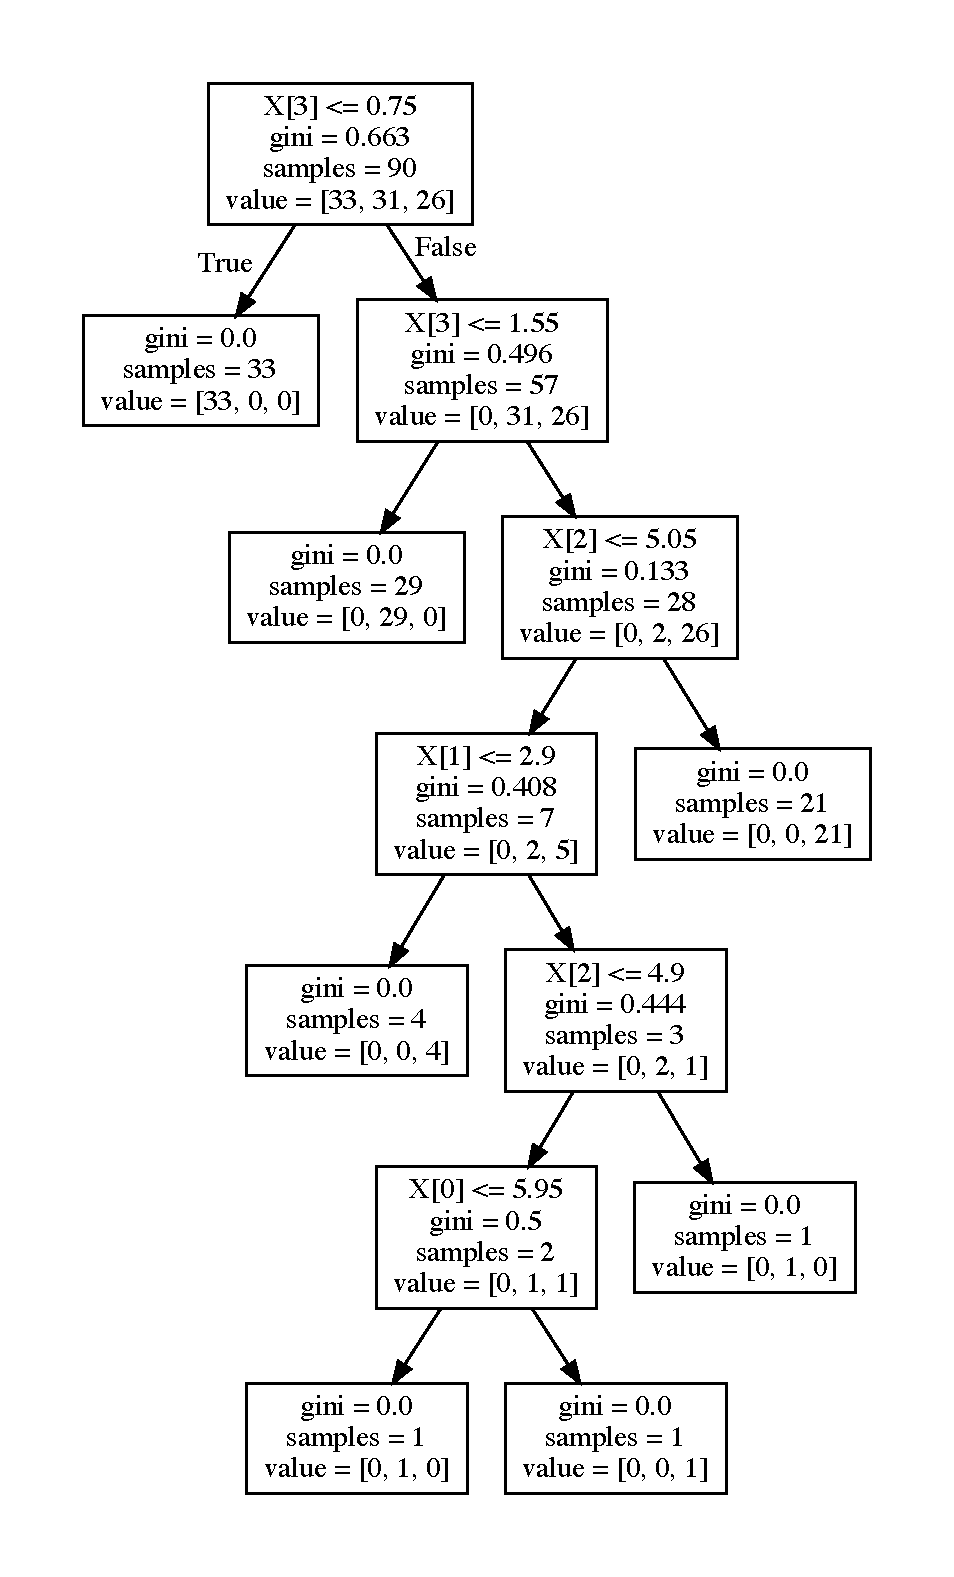
\includegraphics[width=0.8\textwidth]{../figures/iris_decision_tree}
\end{columns}
\end{frame}


\end{document}
